\subsection{Qualitative data}

In the final app test, everyone thought the app was good and easy to use (n = 26). The interview answers of what the coaches said about the app were clustered into areas of Learning, figure \ref{fig:learning}, Interaction Design, figure \ref{fig:interactiondesign}, and Service Design, figure \ref{fig:servicedesign}.

\begin{figure}[h]
    \centering
    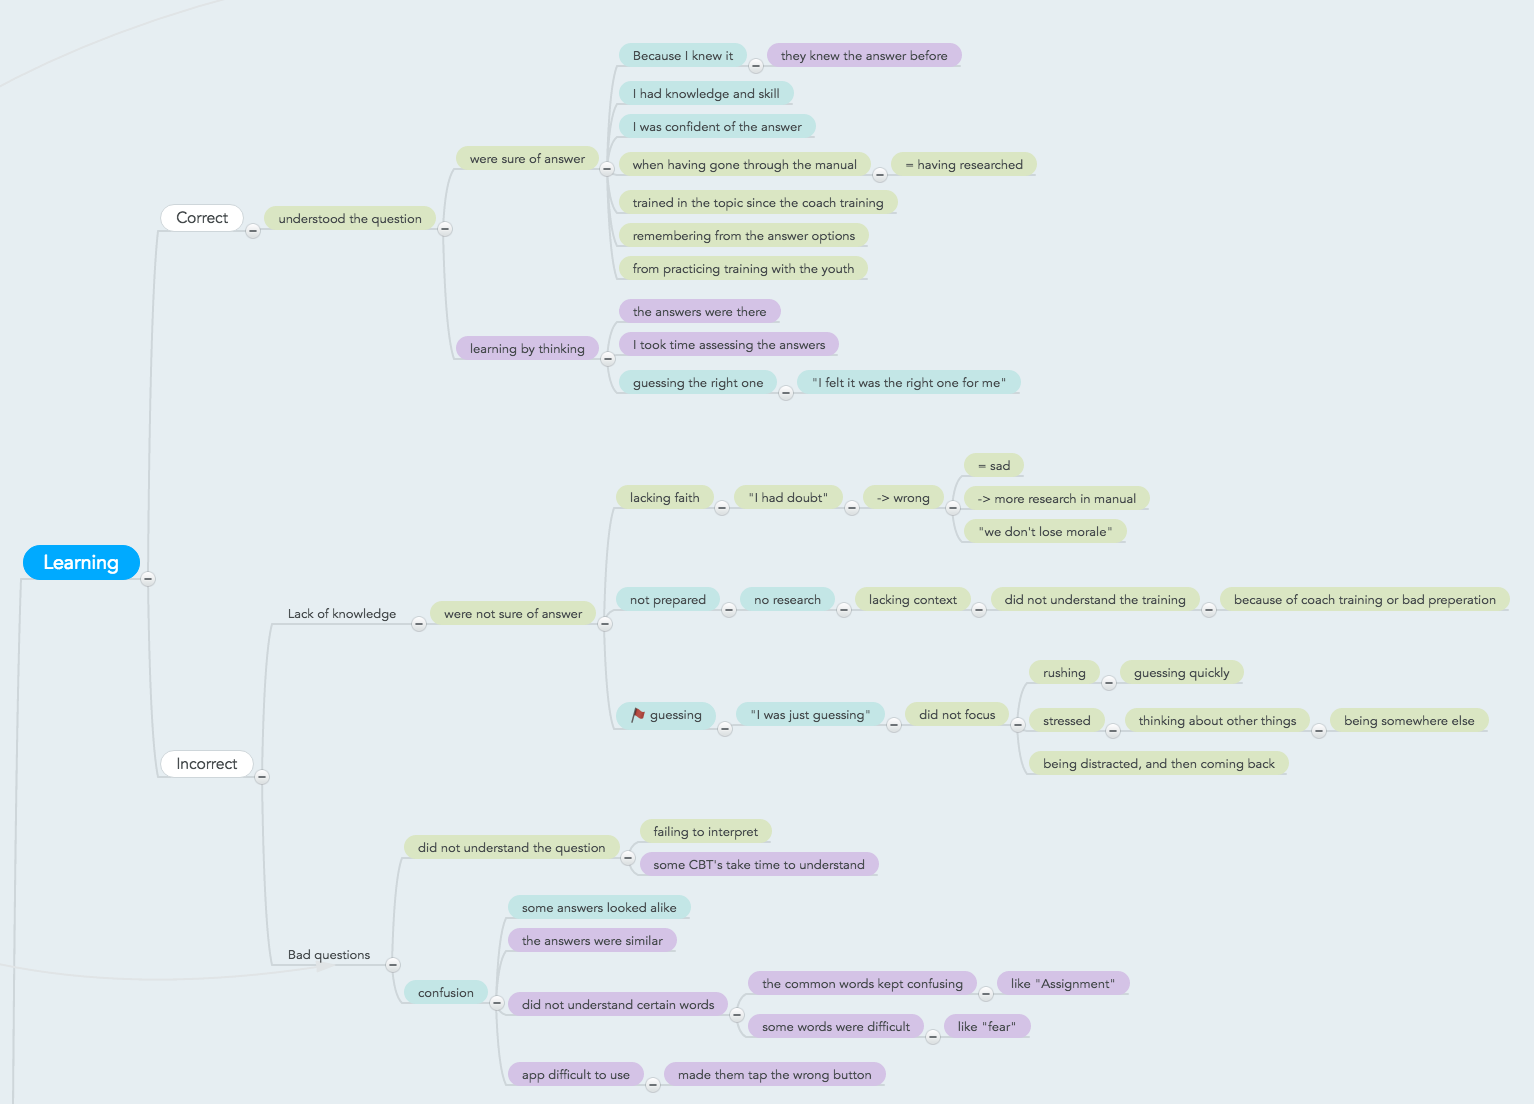
\includegraphics[width=1.0\textwidth]{iteration4qualitative_learning.png}
    \caption{Coach comments regarding learning}
    \label{fig:learning}
\end{figure}

\begin{figure}[h]
    \centering
    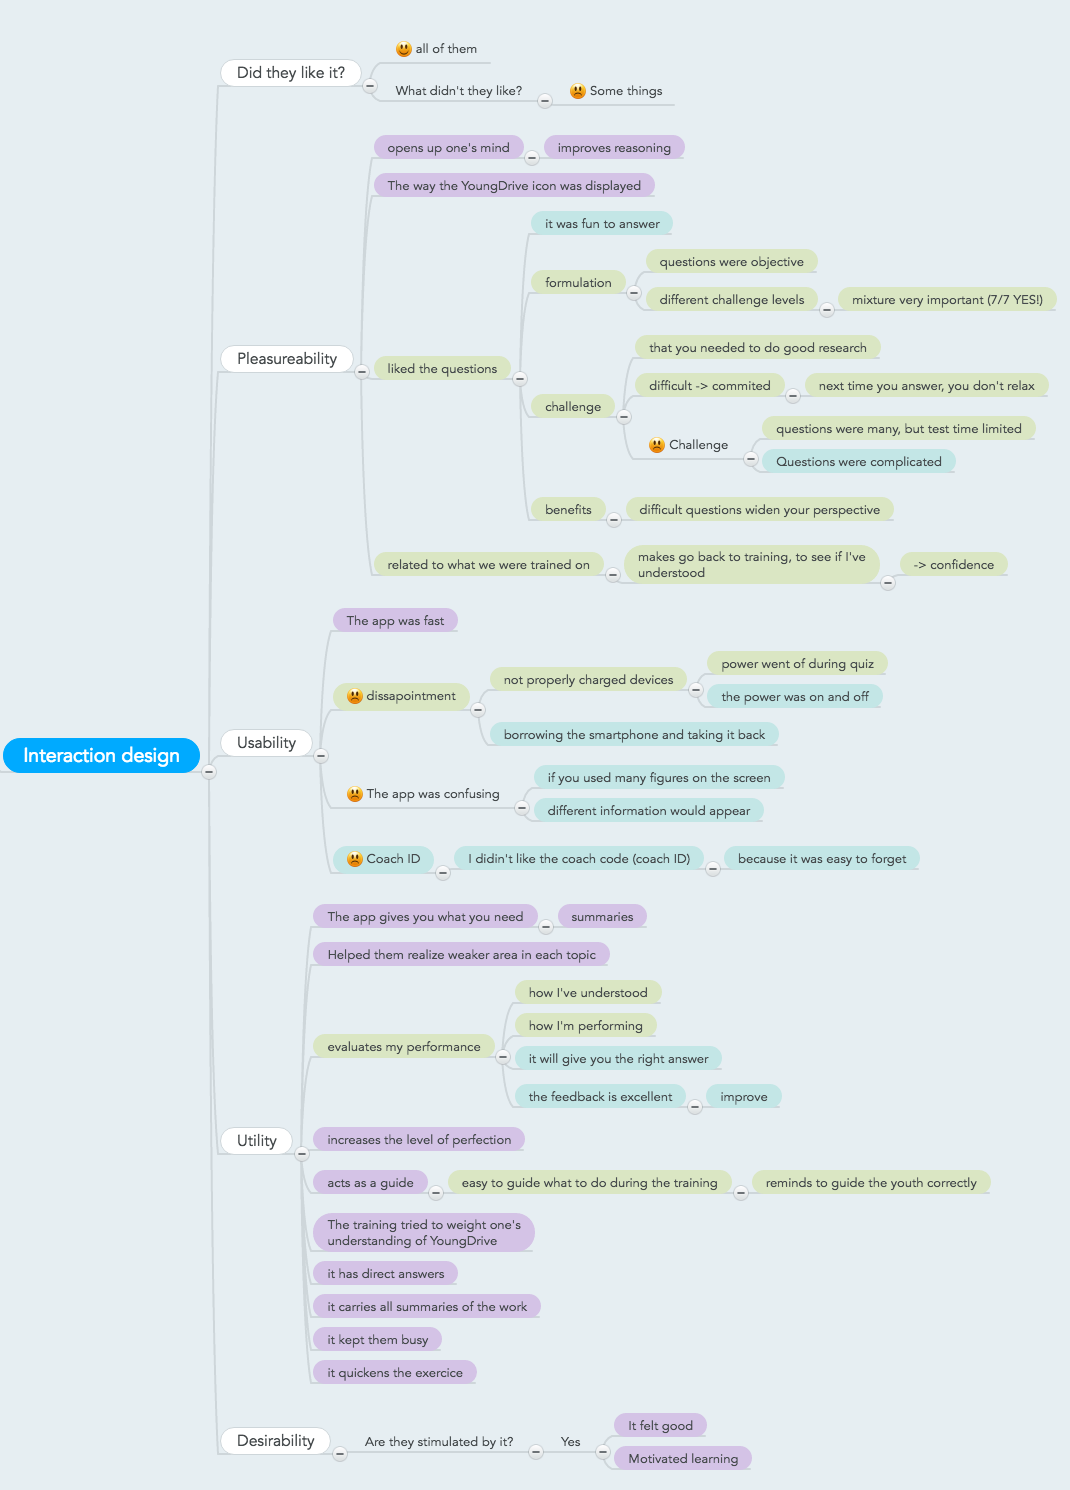
\includegraphics[width=1.0\textwidth]{iteration4qualitative_interactiondesign.png}
    \caption{Coach comments interaction design}
    \label{fig:interactiondesign}
\end{figure}

\begin{figure}[h]
    \centering
    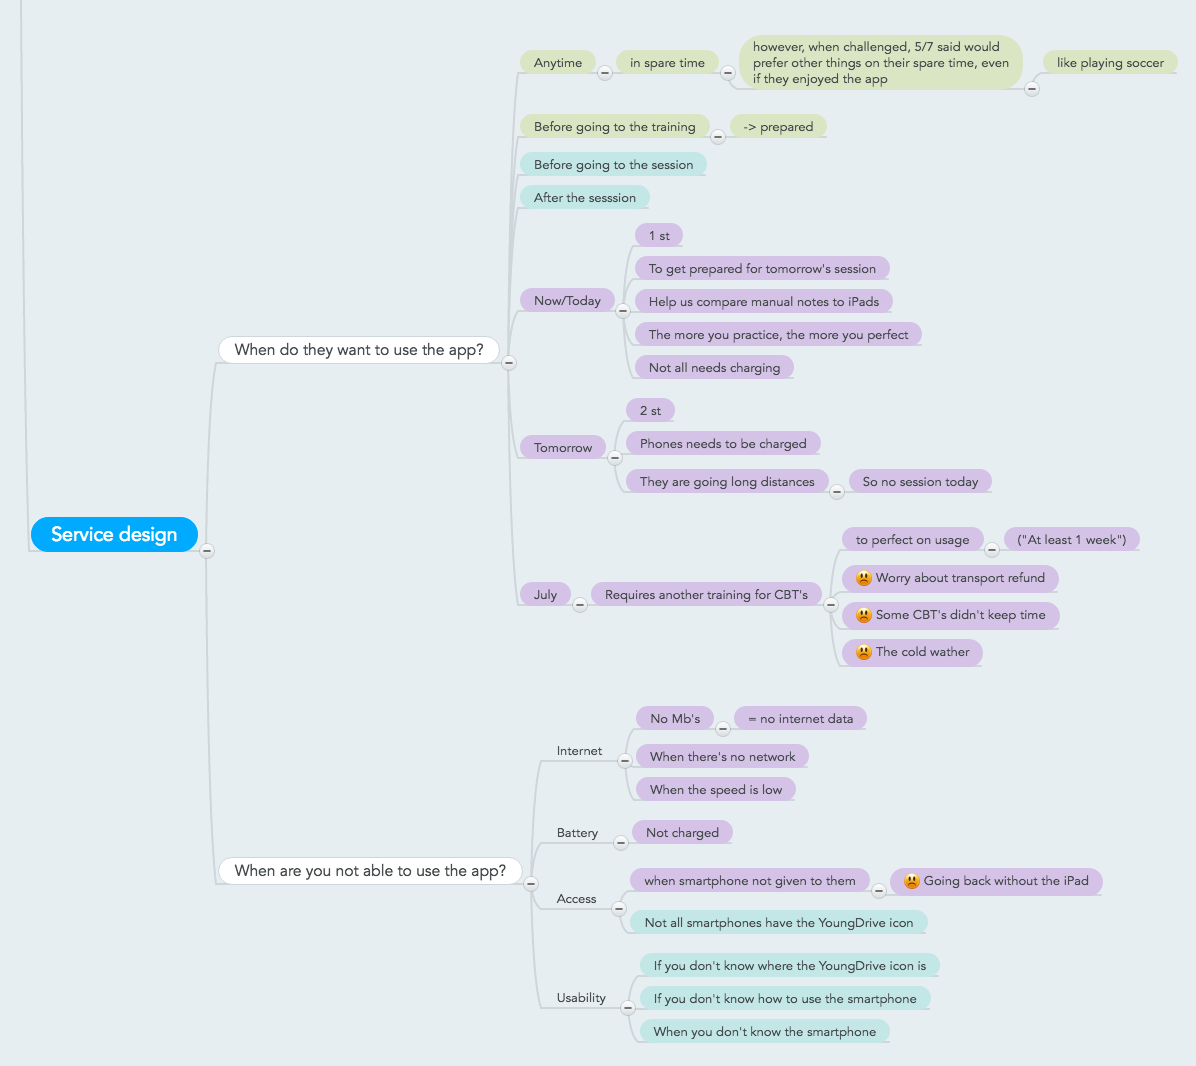
\includegraphics[width=1.0\textwidth]{iteration4qualitative_servicedesign.png}
    \caption{Coach comments regarding service design}
    \label{fig:servicedesign}
\end{figure}

The positive remarks on utility are especially beneficial. The interviews goes in line with than when a coach has passed the certificaiton, they do feel more confident about teaching the topic, since assessment of "Am I ready?" can happen already before the session, and they feel the quiz has been a fair way to measure their knowledge in the topic.
